% Options for packages loaded elsewhere
\PassOptionsToPackage{unicode}{hyperref}
\PassOptionsToPackage{hyphens}{url}
%
\documentclass[
  ,man]{apa6}
\usepackage{amsmath,amssymb}
\usepackage{iftex}
\ifPDFTeX
  \usepackage[T1]{fontenc}
  \usepackage[utf8]{inputenc}
  \usepackage{textcomp} % provide euro and other symbols
\else % if luatex or xetex
  \usepackage{unicode-math} % this also loads fontspec
  \defaultfontfeatures{Scale=MatchLowercase}
  \defaultfontfeatures[\rmfamily]{Ligatures=TeX,Scale=1}
\fi
\usepackage{lmodern}
\ifPDFTeX\else
  % xetex/luatex font selection
\fi
% Use upquote if available, for straight quotes in verbatim environments
\IfFileExists{upquote.sty}{\usepackage{upquote}}{}
\IfFileExists{microtype.sty}{% use microtype if available
  \usepackage[]{microtype}
  \UseMicrotypeSet[protrusion]{basicmath} % disable protrusion for tt fonts
}{}
\makeatletter
\@ifundefined{KOMAClassName}{% if non-KOMA class
  \IfFileExists{parskip.sty}{%
    \usepackage{parskip}
  }{% else
    \setlength{\parindent}{0pt}
    \setlength{\parskip}{6pt plus 2pt minus 1pt}}
}{% if KOMA class
  \KOMAoptions{parskip=half}}
\makeatother
\usepackage{xcolor}
\usepackage{graphicx}
\makeatletter
\newsavebox\pandoc@box
\newcommand*\pandocbounded[1]{% scales image to fit in text height/width
  \sbox\pandoc@box{#1}%
  \Gscale@div\@tempa{\textheight}{\dimexpr\ht\pandoc@box+\dp\pandoc@box\relax}%
  \Gscale@div\@tempb{\linewidth}{\wd\pandoc@box}%
  \ifdim\@tempb\p@<\@tempa\p@\let\@tempa\@tempb\fi% select the smaller of both
  \ifdim\@tempa\p@<\p@\scalebox{\@tempa}{\usebox\pandoc@box}%
  \else\usebox{\pandoc@box}%
  \fi%
}
% Set default figure placement to htbp
\def\fps@figure{htbp}
\makeatother
\setlength{\emergencystretch}{3em} % prevent overfull lines
\providecommand{\tightlist}{%
  \setlength{\itemsep}{0pt}\setlength{\parskip}{0pt}}
\setcounter{secnumdepth}{-\maxdimen} % remove section numbering
% Make \paragraph and \subparagraph free-standing
\makeatletter
\ifx\paragraph\undefined\else
  \let\oldparagraph\paragraph
  \renewcommand{\paragraph}{
    \@ifstar
      \xxxParagraphStar
      \xxxParagraphNoStar
  }
  \newcommand{\xxxParagraphStar}[1]{\oldparagraph*{#1}\mbox{}}
  \newcommand{\xxxParagraphNoStar}[1]{\oldparagraph{#1}\mbox{}}
\fi
\ifx\subparagraph\undefined\else
  \let\oldsubparagraph\subparagraph
  \renewcommand{\subparagraph}{
    \@ifstar
      \xxxSubParagraphStar
      \xxxSubParagraphNoStar
  }
  \newcommand{\xxxSubParagraphStar}[1]{\oldsubparagraph*{#1}\mbox{}}
  \newcommand{\xxxSubParagraphNoStar}[1]{\oldsubparagraph{#1}\mbox{}}
\fi
\makeatother
% definitions for citeproc citations
\NewDocumentCommand\citeproctext{}{}
\NewDocumentCommand\citeproc{mm}{%
  \begingroup\def\citeproctext{#2}\cite{#1}\endgroup}
\makeatletter
 % allow citations to break across lines
 \let\@cite@ofmt\@firstofone
 % avoid brackets around text for \cite:
 \def\@biblabel#1{}
 \def\@cite#1#2{{#1\if@tempswa , #2\fi}}
\makeatother
\newlength{\cslhangindent}
\setlength{\cslhangindent}{1.5em}
\newlength{\csllabelwidth}
\setlength{\csllabelwidth}{3em}
\newenvironment{CSLReferences}[2] % #1 hanging-indent, #2 entry-spacing
 {\begin{list}{}{%
  \setlength{\itemindent}{0pt}
  \setlength{\leftmargin}{0pt}
  \setlength{\parsep}{0pt}
  % turn on hanging indent if param 1 is 1
  \ifodd #1
   \setlength{\leftmargin}{\cslhangindent}
   \setlength{\itemindent}{-1\cslhangindent}
  \fi
  % set entry spacing
  \setlength{\itemsep}{#2\baselineskip}}}
 {\end{list}}
\usepackage{calc}
\newcommand{\CSLBlock}[1]{\hfill\break\parbox[t]{\linewidth}{\strut\ignorespaces#1\strut}}
\newcommand{\CSLLeftMargin}[1]{\parbox[t]{\csllabelwidth}{\strut#1\strut}}
\newcommand{\CSLRightInline}[1]{\parbox[t]{\linewidth - \csllabelwidth}{\strut#1\strut}}
\newcommand{\CSLIndent}[1]{\hspace{\cslhangindent}#1}
\ifLuaTeX
\usepackage[bidi=basic]{babel}
\else
\usepackage[bidi=default]{babel}
\fi
\babelprovide[main,import]{english}
% get rid of language-specific shorthands (see #6817):
\let\LanguageShortHands\languageshorthands
\def\languageshorthands#1{}
\ifLuaTeX
  \usepackage[english]{selnolig} % disable illegal ligatures
\fi
% Manuscript styling
\usepackage{upgreek}
\captionsetup{font=singlespacing,justification=justified}

% Table formatting
\usepackage{longtable}
\usepackage{lscape}
% \usepackage[counterclockwise]{rotating}   % Landscape page setup for large tables
\usepackage{multirow}		% Table styling
\usepackage{tabularx}		% Control Column width
\usepackage[flushleft]{threeparttable}	% Allows for three part tables with a specified notes section
\usepackage{threeparttablex}            % Lets threeparttable work with longtable

% Create new environments so endfloat can handle them
% \newenvironment{ltable}
%   {\begin{landscape}\centering\begin{threeparttable}}
%   {\end{threeparttable}\end{landscape}}
\newenvironment{lltable}{\begin{landscape}\centering\begin{ThreePartTable}}{\end{ThreePartTable}\end{landscape}}

% Enables adjusting longtable caption width to table width
% Solution found at http://golatex.de/longtable-mit-caption-so-breit-wie-die-tabelle-t15767.html
\makeatletter
\newcommand\LastLTentrywidth{1em}
\newlength\longtablewidth
\setlength{\longtablewidth}{1in}
\newcommand{\getlongtablewidth}{\begingroup \ifcsname LT@\roman{LT@tables}\endcsname \global\longtablewidth=0pt \renewcommand{\LT@entry}[2]{\global\advance\longtablewidth by ##2\relax\gdef\LastLTentrywidth{##2}}\@nameuse{LT@\roman{LT@tables}} \fi \endgroup}

% \setlength{\parindent}{0.5in}
% \setlength{\parskip}{0pt plus 0pt minus 0pt}

% Overwrite redefinition of paragraph and subparagraph by the default LaTeX template
% See https://github.com/crsh/papaja/issues/292
\makeatletter
\renewcommand{\paragraph}{\@startsection{paragraph}{4}{\parindent}%
  {0\baselineskip \@plus 0.2ex \@minus 0.2ex}%
  {-1em}%
  {\normalfont\normalsize\bfseries\itshape\typesectitle}}

\renewcommand{\subparagraph}[1]{\@startsection{subparagraph}{5}{1em}%
  {0\baselineskip \@plus 0.2ex \@minus 0.2ex}%
  {-\z@\relax}%
  {\normalfont\normalsize\itshape\hspace{\parindent}{#1}\textit{\addperi}}{\relax}}
\makeatother

\makeatletter
\usepackage{etoolbox}
\patchcmd{\maketitle}
  {\section{\normalfont\normalsize\abstractname}}
  {\section*{\normalfont\normalsize\abstractname}}
  {}{\typeout{Failed to patch abstract.}}
\patchcmd{\maketitle}
  {\section{\protect\normalfont{\@title}}}
  {\section*{\protect\normalfont{\@title}}}
  {}{\typeout{Failed to patch title.}}
\makeatother

\usepackage{xpatch}
\makeatletter
\xapptocmd\appendix
  {\xapptocmd\section
    {\addcontentsline{toc}{section}{\appendixname\ifoneappendix\else~\theappendix\fi: #1}}
    {}{\InnerPatchFailed}%
  }
{}{\PatchFailed}
\makeatother
\keywords{Individual Differences, Reliability, Goodness of Tasks, Hierarchical Models, Experimental Design}
\DeclareDelayedFloatFlavor{ThreePartTable}{table}
\DeclareDelayedFloatFlavor{lltable}{table}
\DeclareDelayedFloatFlavor*{longtable}{table}
\makeatletter
\renewcommand{\efloat@iwrite}[1]{\immediate\expandafter\protected@write\csname efloat@post#1\endcsname{}}
\makeatother
\usepackage{csquotes}
\usepackage{bm}
\usepackage{pcl}
\usepackage{amsmath}
\usepackage{setspace}
\usepackage{mathtools}
\usepackage[table]{xcolor}
\usepackage{bookmark}
\IfFileExists{xurl.sty}{\usepackage{xurl}}{} % add URL line breaks if available
\urlstyle{same}
\hypersetup{
  pdftitle={The Role of Reliability in Experiments},
  pdfauthor={Removed1, Removed1, \& Removed2},
  pdflang={en-EN},
  pdfkeywords={Individual Differences, Reliability, Goodness of Tasks, Hierarchical Models, Experimental Design},
  hidelinks,
  pdfcreator={LaTeX via pandoc}}

\title{The Role of Reliability in Experiments}
\author{Removed\textsuperscript{1}, Removed\textsuperscript{1}, \& Removed\textsuperscript{2}}
\date{}


\shorttitle{Reliability in Experiments}

\authornote{

Version 1, May, 2025.

Correspondence concerning this article should be addressed to Removed. E-mail: Removed

}

\affiliation{\vspace{0.5cm}\textsuperscript{1} Removed\\\textsuperscript{2} Removed}

\abstract{%
Psychological experiments are routinely used to study covariation of individual differences in psychological processes. A key advantage of experimental tasks is that they may offer higher construct validity than traditional survey instruments. Whereas we welcome the generally growing attention to the psychometric evaluation of experimental tasks, we are concerned about an overemphasis on reliability as the principal criterion for evaluating task goodness or interpreting correlations across tasks. In this article, we present a conceptual framework that disentangles three levels of measures: foundational measures of task goodness (i.e., signal-to-noise ratios or intraclass correlations), reliability (which reflects both task goodness and the number of trials), and uncertainty in estimated correlations (which additionally depends on sample size). Within this framework, reliability takes an intermediate position -- it is useful for planning but less so for communicating task goodness or interpreting correlations. Therefore, we advocate for a shift in focus: Researchers should use foundational task goodness measures to communicate the strengths and limitations of experimental designs, and report uncertainty in correlations. To that end, we highlight the role of hierarchical models to jointly estimate trial-level noise and individual variability, thus enabling more accurate and transparent inference about covariation of individual differences.
}



\begin{document}
\maketitle

Cronbach (1957) advocated for combining differential psychology with experimental psychology. One of Cronbach's arguments was that the experimental control in experiments increased construct validity. A good example of this combination of differential and experimental approaches are tasks used in the study of individual differences in executive function. One iconic task is the Stroop Interference Experiment (Stroop, 1935) where words that describes colors, such as \emph{RED,} are displayed in various colors. The participant must report the displayed color, for example, if the word \emph{RED} is displayed in green, the participant must report green and not red. When the display color and word name are incongruent, the task is hard because reading the word is fairly automatic, and it takes executive control to avoid stating red. When they are congruent, for example, the word \emph{RED} is displayed in red, the task is easier and requires little executive control. Hence, the contrast in times between incongruent and congruent items serves to localize executive function, and variations in this contrast across people reflect variations in executive function, and not other factors such as variations in overall speed. It is in this way that experiments have strong construct validity.

Today, it is commonplace to use experiments to explore individual differences in mental abilities The goal in these studies is to explore how experimental tasks covary, for example whether people who have good executive control also perform well on a perceptual discrimination task (Jastrzębski, Kroczek, \& Chuderski, 2021; Tsukahara, Harrison, Draheim, Martin, \& Engle, 2020). In analysis of experiments, researchers tend to borrow heavily from classical test theory. They treat the experiment as a \emph{test} and the mean contrast across conditions per individual as a \emph{score}. Then, scores across various experiments may be correlated and modeled. Experiments, however, differ from more traditional survey instruments in at least the following two ways: (1) As mentioned, in experiments there is often a contrast between conditions and this contrast forms the basis for localization of the process of interest; and (2) experiments are comprised of many trials which are heavily repeated. These differences necessitate a modification to classical-test-theory analysis. The goal of this paper is to describe these differences so that the analysis of individual differences in experiments is more insightful.

The key proposition we advanced here is that the classical concept of reliability has limited use and appeal in experimental contexts. Reliability is useful perhaps in planning experiments, but likely does not play a critical role in interpretation of results.

\section{Why High Reliability?}\label{why-high-reliability}

Sometimes, measurement is critical. For example, people who score well on an abilities tests may be offered admission to medical school; those who score in a pathological range on an autism inventory may be eligible for services, and so on. When measurement is critical in this way, it is equally critical that the measurement be reliable. Without sufficient reliability, it would be too arbitrary to associate resource outcomes with the measurement device.

Reliability has a strong association with classical test theory. In classical test theory, the main unit for analysis is the test itself. Consider, for example, the Beck Depression Inventory II (BDI-II, Beck, Steer, Ball, \& Ranieri, 1996), which is a survey comprised of 21 ratings items.\\
Because the inventory comes complete with a fixed number of items administered in a fixed order with standardized scoring rules, it is reasonable to treat the test as the unit rather than the each of the 21 items separately. The outcome is a single number, the \emph{score.} Moreover, the BDI-II is useful because in part it has good internal reliability, \(\alpha = .91\), and good test-retest reliability, \(r=.93\) (Beck et al., 1996). Experiments, in contrast, do not come in these standardized formats. There is no ``The Stroop Experiment'' with standardized colors, standardized responses, or standardized scoring rules. Most critically, there is no standardized number of replicate trials.

In personality and psychopathology, it is desirable to have reliabilities above .70. The obvious benefit is that highly reliable instruments can be used to make important decisions in good faith. A less obvious benefit of high reliability is that it licenses the study of correlations across measures. Stated briefly, a lack of reliability leads to attenuated correlations (Spearman, 1904). Suppose, for example, we wish to correlate whether depression correlates with working memory, and suppose the instruments have reliability of \(r_1\) and \(r_2\), respectively. Then, even if the depression and working memory correlate fully, the limits on what may be measured are \(\pm \sqrt{r_1r_2}\). If the tasks are highly reliable, say at \(r_1=r_2=.90\), the limits, \(\pm.90\), are close to \(\pm 1\), and the obtained correlation value may be interpreted in a straightforward fashion. If tasks have low reliability, then the observed correlations are limited as well. And when this happens, interpreting correlations is far more difficult.

When using experiments, the goal is often establishing the pattern of correlations across tasks. And, it would seem that high reliability is a precondition for successful analysis. Even so, experiments do not have high reliability in the classical sense. Haaf, Hoffstadt, and Lesche (2024) have cataloged a large corpus of cognitive control studies, and they find reliability around .50 and lower. Moreover, direct comparisons of experiments and survey instruments often find that the surveys are far more reliable. And yet researchers routinely interpret correlations from experiments even when they are greatly attenuated.

\section{Reliability and Signal-To-Noise in Experiments}\label{reliability-and-signal-to-noise-in-experiments}

\subsection{Reliability and Trial Noise}\label{reliability-and-trial-noise}

One issue when measuring the reliability of an experiment is understanding the role of the number of replicate trials. Suppose two labs are each studying the Stroop effect. Each enrolls \(200\) people, and they run identical Stroop tasks with identical colors and response procedures. Both labs run the task on two separate days each, and both compute the correlation of scores across the days as a test-retest reliability index. The only difference between the labs is trial size. Lab A runs \(200\) replicate trials per individual per condition; Lab B runs \(20\) replicate trials per individual per condition. Of course, Lab A has a substantially higher test-retest reliability. We refer to the number of replicate trials per individual per condition as the \emph{trial size} for brevity. Reliability reflects trial size.

Figure \ref{fig:reliability} shows how reliability depends on trial size. The different curves correspond to different experiments. Each curve starts with a reliability of 0 for no trials and reliability increases as trial size is increased. All curves asymptote at 1, and what separates the curves is how fast reliability is gained per added trial. Hence, what characterizes the goodness of the experiment is not the reliability per se but the rate of reliability increase.

\begin{figure}
\centering
\pandocbounded{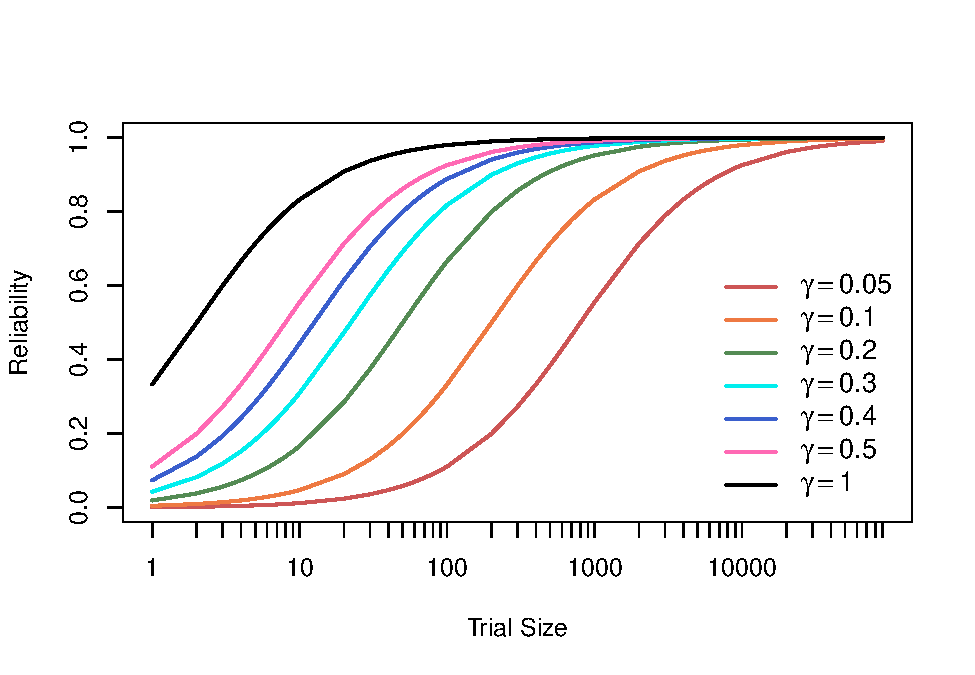
\includegraphics[keepaspectratio]{pBlind_files/figure-latex/reliability-1.pdf}}
\caption{\label{fig:reliability}Reliability as a function of trial size (\(L\)) for different signal-to-noise values (\(\gamma\)). Higher values of \(\gamma\) lead to higher reliability for fewer trials.}
\end{figure}

Some formal development is helpful. Suppose we are performing an experiment with two conditions generically labeled \emph{treatment} and \emph{control}. Each of \(I\) individuals performs \(L\) replicate trials in these two conditions. The observations on each trials are denoted \(Y_{ik\ell}\), where \(i\) denotes the individual, \(i=1,\ldots,I\); \(k\) denotes the condition, \(k=1,2\); and \(\ell\) denotes the replicates, \(\ell=1,\ldots,L\). The usual approach is to compute a contrast score for each individual: \(C_i=\bar{Y}_{i2}-\bar{Y}_{i1}\).

Let's take the simplest model on observations:
\[
Y_{ik\ell} \sim \mbox{Normal}(\alpha_i+x_k\theta_i,\tau^2),
\]
where \(\alpha_i\) is the true overall speed of the \(i\)th individual, \(x_k=-1/2, 1/2\) is a contrast coding, \(\theta_i\) is the contrast score for the \(i\)th individual, and \(\tau^2\) is the degree of trial variability. Parameters \(\alpha_i\) and \(\theta_i\) are \emph{true} parameters because they describe the participants' speed and contrast effect in the limit of increasingly large numbers of trials, respectively. The individual true contrast effect, \(\theta_i\) is the target of inquiry. It is helpful to place a random effects model on this parameter:
\[
\theta_i \sim \mbox{Normal}(\nu,\sigma^2),
\]
where \(\nu\) and \(\sigma^2\) are true population mean and variance parameters, respectively. With the model specified, the distribution on contrast scores is:
\[
C_i \sim \mbox{Normal}\left(\nu,\;\sigma^2+\frac{2\tau^2}{L}\right).
\]

Suppose we repeated an experiment and correlated the contrast scores. The bivariate distribution of the scores is:
\[
\begin{bmatrix} C_{i1} \\ C_{i2}  \end{bmatrix}
\sim \mbox{N}_2 \left(
\begin{bmatrix} \nu \\ \nu  \end{bmatrix},\;
\begin{bmatrix} \sigma^2+\frac{2\tau^2}{L} & \sigma^2 \\
\sigma^2 & \sigma^2+\frac{2\tau^2}{L}
\end{bmatrix}
\right)
\]

The reliability, the correlation between the two instances, denoted \(\rho^*\) is

\begin{eq} \label{eq.reliability}
\rho^* = \frac{\sigma^2}{\sigma^2+2\tau^2/L}.
\end{eq}

The key to understanding the behavior of reliability is to separate the part of the equation that depends on trial size \(L\) from the parts that depend on the variability. This separation is achieved by considering
\begin{equation} \label{gamma2}
\gamma^2=\frac{\sigma^2}{\tau^2}.
\end{equation}
With this substitution,
\[
\rho^* = \frac{\gamma^2}{\gamma^2+2/L}.
\]
We see here that if \(L=0\), the reliability \(\rho^*=0\) and as \(L\) increases, \(\rho^*\) increases as well. In the large trial size limit, \(\rho^*=1\) for all \(\gamma^2\). Reliability is the wrong measure to characterize an experiment because it is not invariant to trial size.

\subsection{Signal-To-Noise Task Goodness Measure}\label{signal-to-noise-task-goodness-measure}

The parameter \(\gamma^2\) is defined in (\ref{gamma2}) as the ratio of between-individual variance and residual trial noise. The numerator, \(\sigma^2\), serves as the \emph{signal} in that if it is large people are easily discriminable. The denominator, \(\tau^2\), is \emph{noise}. Hence, \(\gamma^2\) is the signal-to-noise ratio of an experiment, and it, unlike reliability, can be stated without recourse to trial size (Rouder, Kumar, \& Haaf, 2023).

Rouder and Mehrvarz (2024) advocate \(\gamma^2\) as a task-goodness measure. They ask researchers to report these values and use them for planning trial sizes. They note that (\ref{eq.reliability}) implies:
\[
L=\frac{\frac{2}{\gamma^2}}{\frac{1}{r}-1}.
\]
For example, if \(\gamma^2\approx.02\) and we desire a reliability of .70 or higher, then we must run at least \(L=233\) trials per individual per condition.

Rouder and Mehrvarz (2024) provide the following method-of-moments estimator for a contrast:
\[
\hat{\gamma}^2 = \frac{V_c}{\mbox{MS}_E}-\frac{2}{L},
\]
where \(V_c\) is the variance of observed contrast scores \(C_i\) across individuals and \(\mbox{MS}_E\) is the usual mean square error.

\subsection{Signal-To-Noise For Planning}\label{signal-to-noise-for-planning}

It is helpful to understand the range of signal-to-noise ratios commonly observed in experiments. The Stroop experiment highlighted above tends to have signal-to-noise at about \(\gamma^2=.016\). That is, trial noise is about 64 times greater in variance than the signal we hope to uncover. Here is how: repeated trials in the Stroop task have a standard deviation of about 200 ms give or take. Effects tend to be about 50 ms. The observed standard deviation of these effects is large, but much of this observed value reflects trial noise. After trial noise is accounted for, true effects have about a 25 ms standard deviation, which makes much sense as we do not believe any individual exhibits a true negative Stroop effect where they name incongruent display colors more quickly than congruent ones. The ratio of standard deviations is 25/200; squaring results in \(\gamma^2=.016\). Haaf et al. (2024) in their survey of 64 cognitive control experiments find this value as an average, and values typically range from .005 to .0625. Clearly, many trials are needed in cognitive control studies if individual differences are going to be effectively localized.

\subsection{Signal-To-Noise And Intraclass Correlation}\label{signal-to-noise-and-intraclass-correlation}

The signal-to-noise ratio, \(\gamma^2\), is closely related to the intraclass correlation coefficient (ICC). There are several ICC measures, and the appropriate one here is ICC(1) (see McGraw \& Wong, 1996). ICC is typically considered a descriptive statistic and it is typically not applied to design without contrasts. Let's take the following as the base model where there are no conditions to contrast: \(Y_{i\ell}\sim \mbox{N}(\theta_i,\tau^2)\) with \(\theta_i\sim \mbox{N}(\nu,\sigma^2)\). In this case, researchers compute \(\bar{Y}_i\) as the score. The question then is how \(\gamma^2\) relates to ICC(1) for this case.

McGraw and Wong (1996) note that ICC(1) is an estimate of \(\kappa\):
\[
\kappa = \frac{\sigma^2}{\sigma^2 + \tau^2}.
\]
Substituting in for \(\gamma^2\) reveals \(\kappa=\gamma^2/(1+\gamma^2)\), or that \(\gamma^2\) is the odds form of \(\kappa\).

Let's compare estimators. The estimator of \(\gamma^2\) in this case without contrasts is
\[
\hat{\gamma}^2=\frac{V}{\mbox{MS}_E}-\frac{1}{L},\quad
V=\frac{\sum_i (\bar{Y}_i-\bar{Y})^2}{(I-1)}.
\]

McGraw and Wong (1996){]} recommend computing ICC(1) from a one-way ANOVA as
\[
\mbox{ICC(1)}=\frac{\mathrm{MS}_R - \mathrm{MS}_E}{\mathrm{MS}_R + (L - 1)\mathrm{MS}_E,}
\]\\
where \(\mathrm{MS}_R = L\times V\). It is straightforward to show that \(\mbox{ICC}(1) = \frac{\hat{\gamma}^2}{\hat{\gamma}^2 + 1}\). Hence \(\gamma^2\) and ICC(1) are simply different parameterizations of the same core quantity. We find the signal-to-noise ratio a bit more facile as a communication device, but that might reflect personal familiarity and ease more than anything else. Both \(\gamma^2\) and \(\kappa\) are capturing the same information albeit in different forms. They may be used interchangeably. Most importantly, both are superior to reliability as a task-goodness measure.

\section{Low Reliability and Misplaced Certainty in Low Correlations}\label{low-reliability-and-misplaced-certainty-in-low-correlations}

When practitioners score an individual with an instrument, the goal may be to learn about that individual so that appropriate resources may be allotted. In experiments, in contrast, the usual goal is to correlate individual differences across a variety of tasks. Experimenters ask questions such as ``are perceptual abilities related to working memory?'' It is well known that low reliability leads to attenuated correlations. What is less well known---at least among experimentalists---is that it leads to dramatic overconfidence in what is learned. The resulting CIs are far too narrow and rarely cover the true values.

Let's expand the model for multiple experimental tasks. Let \(j=1,2\) index two such tasks, and let \(Y_{ijk\ell}\) denote an observation for the \(i\)th individual, \(j\)th task, \(k\)th condition, and \(\ell\)th replicate:
\[
Y_{ijk\ell} \sim \mbox{Normal}(\alpha_{ij}+x_k\theta_{ij},\tau_j^2)
\]
We place a random effects model on true effects as before, but allow correlation \(\rho\) across the tasks:
\[
\begin{bmatrix} \theta_{i1} \\ \theta_{i2} \end{bmatrix} \sim \mbox{N}_2 \left( \begin{bmatrix} \nu_1 \\ \nu_2 \end{bmatrix}, \begin{bmatrix}
\sigma_1^2 & \rho \sigma_1 \sigma_2 \\
\rho \sigma_1 \sigma_2 & \sigma_2^2
\end{bmatrix}\right)
\]

We are now in position to simulate data and see how we can recover \(\rho\). The usual approach is to compute contrasts \(C_{ij}\) for each individual in each task, that is, \(C_{ij} = \bar{Y}_{ij2}-\bar{Y}_{ij1}\). Then the sample correlation across the two tasks is computed, and confidence intervals may be attained conventionally through Fisher's \(z\)-transform method (Fisher, 1921; Fisher, 1915).

We ran simulations from the above model. For both tasks \(L=100\), \(\tau=.175\), \(\sigma=.025\) and \(\rho=.5\). These are reasonable values, and each task has a signal-to-noise ratio \(\gamma^2=.02\), which is pretty sizable for typical cognitive-control tasks. We varied \(I\) and plotted the obtained correlation coefficient and associated 95\% CIs for 100 replicate data sets.

\begin{figure}
\centering
\pandocbounded{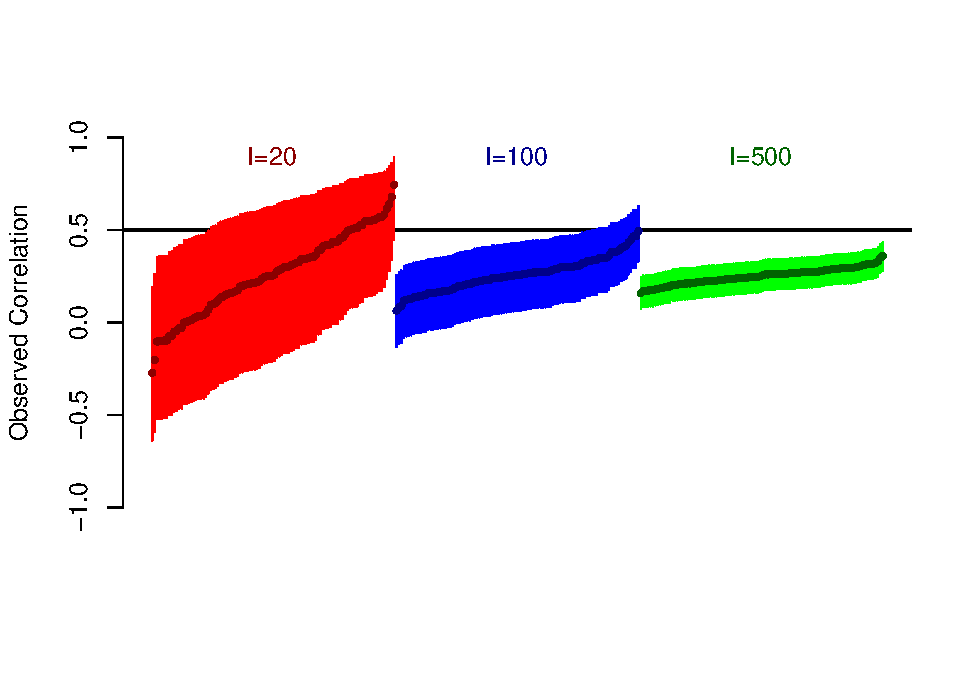
\includegraphics[keepaspectratio]{pBlind_files/figure-latex/obsCor-1.pdf}}
\caption{\label{fig:obsCor}Confidence interval coverage from simulated data with known ground truth. The figure shows 100 simulations for each of three setups. In each setup, task signal-to-noise was \(\gamma=.143\) and each individual performed 100 trials in each of two conditions per task. The three setups have, respecitvely, \(I=20\), \(I=100\), and \(I=500\) individuals. Confidence intervals are denoted with vertical lines, and these come from Fisher's z-transform on sample correlations. These intervals are woefully miscalibrated failing to cover the true correlation in a majority of runs. Even worse, coverage decreases with increasing numbers of individuals.}
\end{figure}

Figure \ref{fig:obsCor} shows the results for sample sizes of \(I=20\), \(I=100\), and \(I=500\). The trend is clear. Not only is the observed correlation biased below the true value of .50, the CIs do not cover it as well. If our goal is to measure \(\rho\), we have entered a bit of a statistical hell. The estimator is \emph{inconsistent} with respect to increasing numbers of individuals. As more individuals are added to the design, the attenuation does not abate. One becomes more certain of a wrong value.

Experimentalists who use individual differences routinely tout their large sample sizes that cover several hundred individuals. They routinely compute contrast scores across these great many people, and correlate these contrast scores across tasks. They star those that are significant without acknowledgment that the significance test is based on such a faulty sense of uncertainty.

\section{A Focus on Uncertainty}\label{a-focus-on-uncertainty}

Correlations serve as the main target when using experiments to understand individual differences. And when estimating them, our target should be the true correlation among individuals across experimental tasks as if there were an unlimited number of trials, that is what is denoted \(\rho\) rather than \(\rho^*\) in the preceding development. In estimating \(\rho\), we should strive for two desiderata. The first is \textbf{consistency} in estimation with respect to increasing numbers of individuals. As this number becomes larger, the estimate should become more accurate and, in the limit, achieve the true value with certainty. The second desideratum is an \textbf{accurate assessment of uncertainty.} The associated error bars or confidence intervals should accurately quantify the uncertainty in estimation. Sample correlations fail dramatically to meet these desiderata. One is too certain in an attenuated value.

The solution to these problems is to model trial noise in a mixed-model setup. Here is a simple, flexible hierarchical model for analysis. The model has a data component and a latent component. Let \(\bfY_{ij}\) be a vector of \(n_{ij}\) observations for the \(i\)th person in the \(j\)th experimental task:
\[
\bfY_{ij} \sim \mbox{N}_{n_{ij}}(\bfX_{0ij}\bfalpha_{ij}+\bfX_{1ij}\theta_{ij},\;\tau_j^2\bfI).
\]
Distribution \(N_{n_{ij}}\) is a multivariate normal of dimension \(n_{ij}\), that is the dimension of the number of observations. The main target is latent ability \(\theta_{ij}\). \(\bfX_{1ij}\) is a column vector of length \(N_{ij}\) that describes how \(\theta_{ij}\) affects observations. \(\bfalpha_{ij}\) is a vector of additional latent individual parameters and \(\bfX_{0ij}\) describes how these parameters affect observations. For example, if the first task (\(j=1\)) is a Stroop task with congruent and incongruent conditions, then \(\bfX_{0i1}\) is a vector of 1's; \(\alpha_{i1}\) is a parameter for overall speed, \(\bfX_{1i1}\) is a vector with values of \(-1/2\) and \(1/2\) for congruent and incongruent trials, respectively, and \(\theta_{i1}\) is the Stroop effect. Trial variability is task specific but homogeneous across individuals, conditions, and replicates.

The next level is the latent level, and a model is specified for effects \(\theta_{ij}\). To capture covariation, let \(\bftheta_i=(\theta_{i1},\ldots,\theta_{iJ})'\) be a column vector of latent abilities for the \(J\) experimental tasks:

\[
\bftheta_i \sim \mbox{N}_J(\bfmu,\bfSigma).
\]

In fact, we may rewrite this variance as
\[
\bfSigma=D(\bfsigma^2)\bfrho D(\bfsigma^2),
\]
where \(D(\bfsigma^2)\) is a diagonal matrix with a diagonal of \(\bfsigma^2=(\sigma_1^2,\ldots,\sigma_J^2)\) of variances and \(\bfrho\) a correlation matrix of correlations across tasks. Signal-to-noise ratios \(\gamma^2_j\) remain \(\gamma^2_j = \sigma^2_j/\tau^2_j\).

The model is a standard hierarchical model, and analysis is convenient in frequentist or Bayesian frameworks. We personally prefer the Bayesian approach for two reasons: First, it is conceptually straightforward and computationally convenient. Second, it is particularly straightforward to analyze the propagation of uncertainty from the prior to the posterior. This is not to say that implementation must be Bayesian or is even better as Bayesian; it is just our preference to work here.

How does the model perform? We took a run from the previous simulation as data where \(I=100\) and the true correlation is .50 in value. Figure \ref{fig:example} shows the results from sample statistics and from model analysis. The left panel shows the observed contrast scores for the first task ordered from smallest to largest as points (``+''). The blue intervals and points are model effects \(\theta_i\) for the first task using the order on contrast scores. Two features are evident. First, there is much shrinkage indicating that most of the observed variability in the contrast score reflects trial noise. Second, there are small perturbations or wiggles where the model effect does not exactly track the contrast score. These wiggles are not noise in MCMC sampling but reflect the workings of the model. The wiggles are the influence of the effects in the second task.

The right panel shows the estimates of correlation. The true value of .50 is indicated by the thick vertical line. The correlation of observed contrasts is shown as the dark red point; the horizontal error bars show the 95\% confidence interval. As noted previously, the value is too small and the interval is too small to cover the true value. The prior for the model correlation is the uniform density; the posterior from MCMC samples is shown as a histogram. The posterior mean is .56 which is quite close to the true value. There is much posterior uncertainty, however.

\begin{figure}
\centering
\pandocbounded{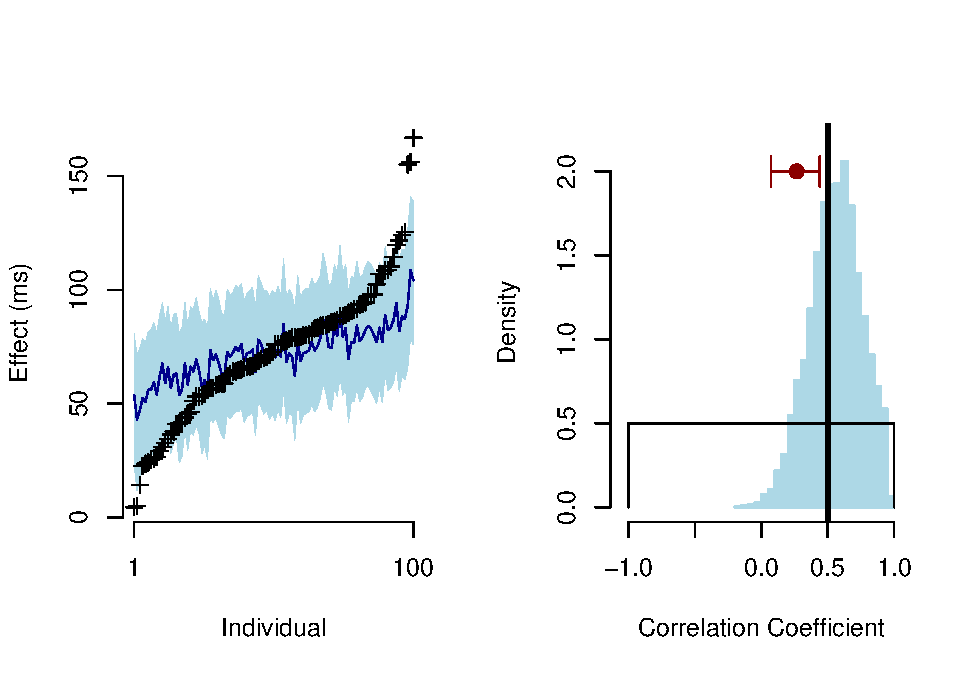
\includegraphics[keepaspectratio]{pBlind_files/figure-latex/example-1.pdf}}
\caption{\label{fig:example}Model outputs. A. The points (plusses) are observed individual effects ordered from smallest to largest for one of the two tasks. The solid line is the corresponding model point estimate; the shaded area is the corresponding 95\% credible interval. There is a large degree of regularization indicating that much of the variability in the observed scores is due to trial noise. B. The histogram shows the posterior distribution of the correlation coefficient. The thick vertical line is the true value, and it is well within the posterior. The red point with confidence intervals is the observed correlation. It is attenuated and the CIs do not cover the true value.}
\end{figure}

How to interpret this posterior uncertainty? The 95\% credible interval from the posterior is {[}0.16,0.91{]}, the width of which is 0.75. We can compare this to the smaller interval from the correlation among observed contrasts, which is only 0.37 in width. The width of this interval reflects only the value of the correlation and the number of individuals \(I\). In this sense, it reflects to large degree the uncertainty from a finite sample of individuals. Indeed, if there were a great many trials, the posterior uncertainty in the hierarchical model would approach this width. The additional width in the hierarchical posterior reflects the uncertainty from a finite number of trials. This is the appropriate measure researchers should convey when assessing the importance of correlations---it reflects the true limitations of the design.

\section{Reliability Is No Longer Important For Interpreting Experiments}\label{reliability-is-no-longer-important-for-interpreting-experiments}

The story has now come full circle. High reliability is sought because the correlation among highly-reliable instruments may be interpreted without concern. Experiments, in contrast, are rarely highly reliable, but that fact has not prevented researchers from exploring correlations among tasks. We have shown here that disattenuation is only part of the problem in interpretation---the other part is that uncertainty in conventional correlations are understated leading to overstated confidence in attenuated values.

Once we agree that it is critical to appropriately express uncertainty from finite samples of individuals and trials, then reliability is tangential. Correlations may be interpreted within their uncertainty and without recourse to reliability. And, since we can assess uncertainty in correlations directly by modeling trial noise, we can state (increased) uncertainty even in low reliability designs. The old adage that you can't correlate unreliable instruments is not true with experiments. You can do so, leveraging the information in repeated trials, so long as uncertainty is appropriately assessed. The bottom line is with these hierarchical models, reliability is not needed for estimation or interpretation.

\section{Reliability in Planning Experiments}\label{reliability-in-planning-experiments}

There is one area where reliability still plays an outsized role: planning.
It is unpleasant to discover after the fact---after much time and energy in data collection---that a posterior correlation is poorly localized. And it would be valuable to have planning tools so researchers know what numbers of individuals and trials are needed before data collection.

The most convenient setup for planning is to assume that the true correlation is 0 in value. Not only is this the worst-case in that credible intervals are widest, it is also the easiest to understand analytically. What we seek is a function, denoted \(w(I,L_1,L_2,\gamma^2_1,\gamma^2_2)\) that provides the width of the 95\% credible interval on a truly null correlation between two tasks.

Let's start with the boundary case where there is no trial noise. This boundary case is achieved either as trial noise goes to 0 (\(\gamma^2 \rightarrow \infty\)) or the trials are increased (\(L\rightarrow \infty\)).
The width of the credible intervals may be obtained through classical methods including Fisher's \(z\)-transformation (Fisher, 1921). The expected width for a true correlation of zero, denoted \(s_{95}(I)\), is:
\[
s_{95}(I) \approx \tan^{-1}\left(\frac{1.96}{\sqrt{I-3}}\right)-\tan^{-1}\left(\frac{-1.96}{\sqrt{I-3}}\right)
\]

This width serves as a lower bound and best case. The question then is how much is it inflated by finite trial sizes and trial noise. A key quantity is the attenuation factor of correlations from trial noise, which is:
\[
a(L_1,L_2,\gamma_1,\gamma_2)=\sqrt{\frac{\gamma_1^2}{(\gamma_1^2+2/L_1)}\frac{\gamma_2^2}{(\gamma_2^2+2/L_2)}},
\]
where \(0 \leq a \leq 1\) and \(a=1\) corresponds to no trial noise and \(a=0\) corresponds to infinitely large trial noise. Confidence intervals increase not decrease with increasing trial noise, and the appropriate expansion factor is \(1/a\). For planning, and as a rough guide, we recommend researchers compute:

\begin{equation}
\label{approx}
w(I,L_1,L_2,\gamma^2_1,\gamma^2_2) \approx \frac{s(I)}{a(L_1,L_2,\gamma_1,\gamma_2)}.
\end{equation}

We can re-express the attenuation in terms of the expected reliability of tasks. This expected reliability, \(r\), is:
\[
r = \frac{\gamma^2}{(\gamma^2+2/L)}.
\]
With this, the width function can also be expressed in terms of reliability:
\[
w(I,r_1,r_2) \approx s(I)\times \sqrt{r_1r_2}.
\]

Of course, actual credible intervals (and confidence intervals) are random variables and functions of observables. To show how these credible intervals may vary in real data, we performed a set of simulations. We factorially manipulated \(I\) (100, 200), \(L\) (50, 100, 200, 400), and \(\gamma\) (0, .1, .2, .5) for each of two tasks. At the population level, the tasks were not correlated. Then we generated true individual scores and from these trial-level data. Sample correlations with associated CIs were computed, and the width of these is \(s\). The data were also submitted to hierarchical model analysis, and posterior 95\% credible intervals (width of \(w\)) on the correlation coefficient were estimated. For each combination of \(I\), \(L\) and \(\gamma\), the cycle of sampling true values, sampling trial-level data, and analysis was repeated 1000 times.

The results of the simulation are shown in Figure \ref{fig:sims}. The left panel shows the ratio \(w/s\), termed the \emph{Width Ratio} as a function of \(1/a\), termed the \emph{Expansion Factor}. The median is shown as the black line, and indeed, it is very close to the diagonal. The 10\% and 90\% of the ratios are also shown, and these deviate in a reasonable fashion from the diagonal.

\begin{figure}
\centering
\pandocbounded{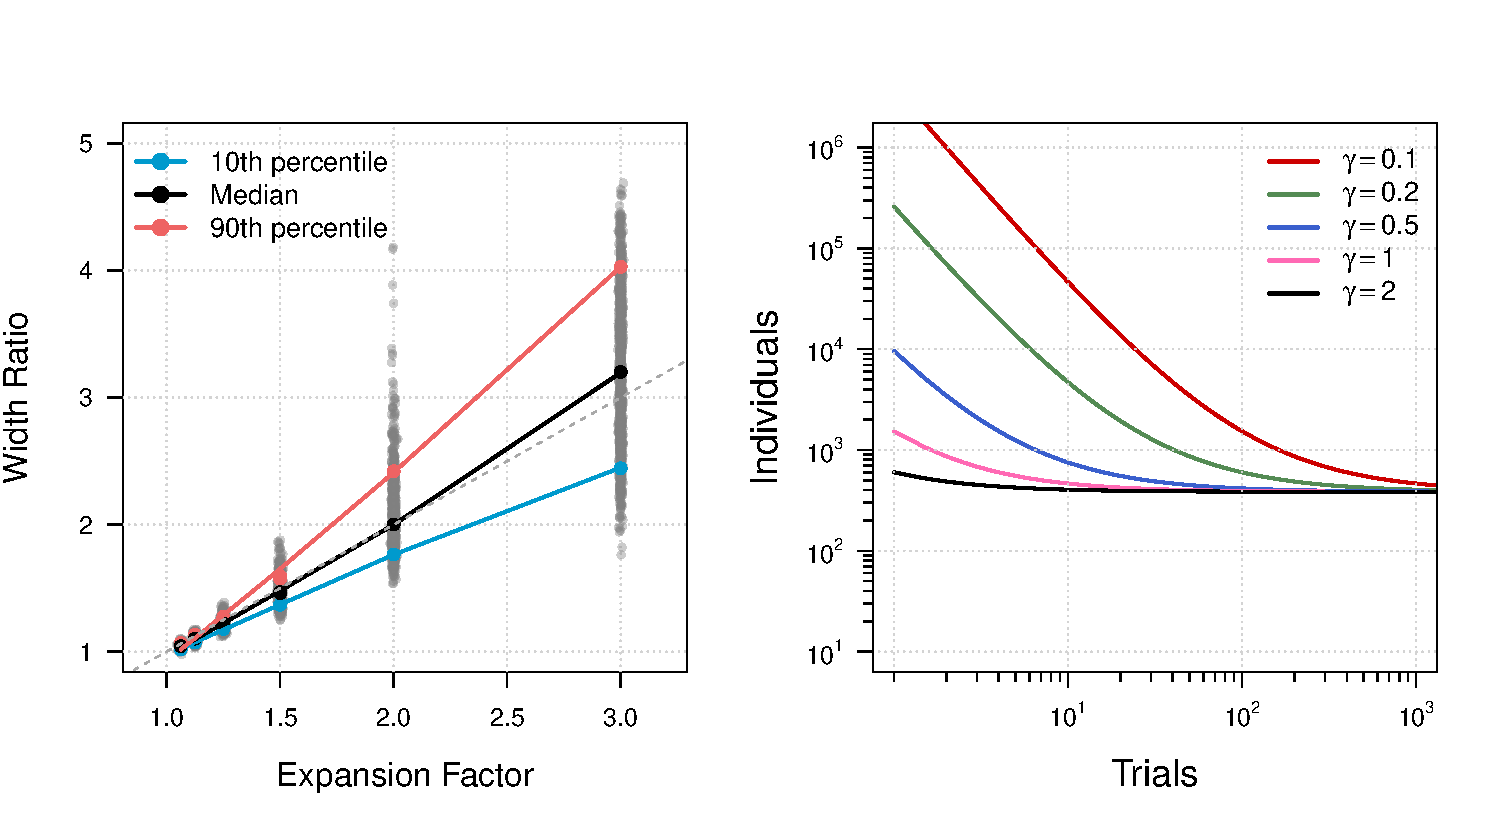
\includegraphics[keepaspectratio]{pBlind_files/figure-latex/sims-1.pdf}}
\caption{\label{fig:sims}Planning for trial noise. A. Width ratio as a function of expansion factor. Width ratio is expansion of uncertainty when taking into account trial noise and is measured as the ratio of the posterior credible interval width to the sample confidence interval width (\(w/s\)). Exapansion factors are the reciprocal of the geometric mean of task reliability (\(1/a\)). The figure shows the case for \(\gamma=.2\) across a variety of trial sizes (\(L\)) and sample sizes (\(I\)). Gray dots are simulation replicates; the solid lines mark the 10th, 50th, and 90th percentiles across replicates. B. Tradeoff of trial size \(L\) and \(I\) needed to acheive a target credible interval with of \(.2\) in value for different signal-to-noise ratio values (\(\gamma\)).}
\end{figure}

\section{Discussion}\label{discussion}

Psychological experiments are often used to measure individual variation in abilities. These experiments, because they rely on contrasts between conditions, may have higher construct validity than more traditional survey measures. Unfortunately, they are associated with low reliability, and this low reliability comes about because individual differences in contrasts may be less stable than hoped (Draheim, Tsukahara, Martin, Mashburn, \& Engle, 2021).

In our view, this low reliability, while consequential, is not the appropriate way of understanding measurement noise or its affects in assessing correlations. We provide a view where reliability is neither used for communication about task goodness nor in the assessment of uncertainty. It's role is more relevant for planning.

Figure \ref{fig:overall} shows how reliability fits into conceptualizing individual differences with experiments. At the left are foundational measures of task goodness that are portable in that they hold for any number of trials or individuals (Rouder \& Haaf, 2019). Reliability reflects this information as well as considerations of trial size. Correlations among tasks is further up stream, and reflects both reliability and the number of individuals. In this sense, reliability is semi-portable, one must commit to a specific trial size but not to a number of individuals. Uncertainty in correlations, the critical output for assessing the significance of a correlation, reflects all factors: task goodness, trial size, and the number of people. And once we make this explicit, reliability is just a midway point.

\begin{figure}

{\centering 
\includegraphics[width=1\linewidth]{planning} 

}

\caption{Analysis begins with measures of task goodness that are invariant to trial size $L$ and sample size $I$.  Suitable measures are signal-to-noise and ICC(1).  Reliability and attenuation factors reflect task goodness and trial size $L$ but not sample size $I$.  Uncertainty on correlations reflects reliability and the number of individuals $I$.  In this sense, reliability sits between task goodness and correlation precision---incorporating trial size but not sample size.}\label{fig:overall}
\end{figure}

In summary, we recommend that researchers focus on reporting uncertainty in correlations and communicate in task goodness measures about the advantages and disadvantages of various tasks. Hierarchical models are invaluable in implementing these recommendations as they allow the simultaneous modeling of trial noise and individual variability.

\newpage

\section*{References}\label{references}
\addcontentsline{toc}{section}{References}

\phantomsection\label{refs}
\begin{CSLReferences}{1}{0}
\bibitem[\citeproctext]{ref-Beck.etal.1996}
Beck, A. T., Steer, R. A., Ball, R., \& Ranieri, W. (1996). Comparison of {Beck Depression Inventories} -{IA} and -{II} in psychiatric outpatients. \emph{Journal of Personality Assessment}, \emph{67}(3), 588--597. doi:\href{https://doi.org/10.1207/s15327752jpa6703_13}{10.1207/s15327752jpa6703\_13}

\bibitem[\citeproctext]{ref-Cronbach.1957}
Cronbach, L. J. (1957). The two disciplines of scientific psychology. \emph{American Psychologist}, \emph{12}(11), 671--684. doi:\href{https://doi.org/10.1037/h0043943}{10.1037/h0043943}

\bibitem[\citeproctext]{ref-Draheim.etal.2021}
Draheim, C., Tsukahara, J. S., Martin, J. D., Mashburn, C. A., \& Engle, R. W. (2021). A toolbox approach to improving the measurement of attention control. \emph{Journal of Experimental Psychology: General}, \emph{150}(2), 242. doi:\href{https://doi.org/10.1037/xge0000783}{10.1037/xge0000783}

\bibitem[\citeproctext]{ref-Fisher.1921}
Fisher, R. (1921). On the {``{Probable Error}''} of a {Coefficient} of {Correlation Deduced} from a {Small Sample}. \emph{Metron}, \emph{1}, 3--32.

\bibitem[\citeproctext]{ref-Fisher.1915}
Fisher, R. A. (1915). Frequency {Distribution} of the {Values} of the {Correlation Coefficient} in {Samples} from an {Indefinitely Large Population}. \emph{Biometrika}, \emph{10}(4), 507--521. doi:\href{https://doi.org/10.2307/2331838}{10.2307/2331838}

\bibitem[\citeproctext]{ref-Haaf.etal.2024}
Haaf, J. M., Hoffstadt, M., \& Lesche, S. (2024). Attentional {Control Data Collection}: {A Resource} for {Efficient Data Reuse}. doi:\href{https://doi.org/10.31234/osf.io/4evy6}{10.31234/osf.io/4evy6}

\bibitem[\citeproctext]{ref-Jastrzebski.etal.2021}
Jastrzębski, J., Kroczek, B., \& Chuderski, A. (2021). Galton and {Spearman} revisited: {Can} single general discrimination ability drive performance on diverse sensorimotor tasks and explain intelligence? \emph{Journal of Experimental Psychology: General}, \emph{150}(7), 1279--1302. doi:\href{https://doi.org/10.1037/xge0001005}{10.1037/xge0001005}

\bibitem[\citeproctext]{ref-McGraw.Wong.1996}
McGraw, K. O., \& Wong, S. P. (1996). Forming inferences about some intraclass correlation coefficients. \emph{Psychological Methods}, \emph{1}(1), 30. Retrieved from \url{https://psycnet.apa.org/journals/1082-989X/1/1/30/}

\bibitem[\citeproctext]{ref-Rouder.Haaf.2019}
Rouder, J. N., \& Haaf, J. M. (2019). A psychometrics of individual differences in experimental tasks. \emph{Psychonomic Bulletin and Review}, \emph{26}(2), 452--467. Retrieved from \url{https://doi.org/10.3758/s13423-018-1558-y}

\bibitem[\citeproctext]{ref-Rouder.etal.2023}
Rouder, J. N., Kumar, A., \& Haaf, J. M. (2023). Why many studies of individual differences with inhibition tasks may not localize correlations. \emph{Psychonomic Bulletin \& Review}, \emph{30}(6), 2049--2066. doi:\href{https://doi.org/10.3758/s13423-023-02293-3}{10.3758/s13423-023-02293-3}

\bibitem[\citeproctext]{ref-Rouder.Mehrvarz.2024}
Rouder, J. N., \& Mehrvarz, M. (2024). Hierarchical-{Model Insights} for {Planning} and {Interpreting Individual-Difference Studies} of {Cognitive Abilities}. \emph{Current Directions in Psychological Science}, \emph{33}(2), 128--135. doi:\href{https://doi.org/10.1177/09637214231220923}{10.1177/09637214231220923}

\bibitem[\citeproctext]{ref-Spearman.1904a}
Spearman, C. (1904). The {Proof} and {Measurement} of {Association} between {Two Things}. \emph{American Journal of Psychology}, \emph{15}, 72--101. Retrieved from \url{https://www.jstor.org/stable/pdf/1412159.pdf?refreqid=excelsior\%3Af2a400c0643864ecfb26464f09f022ce}

\bibitem[\citeproctext]{ref-Stroop.1935}
Stroop, J. R. (1935). Studies of interference in serial verbal reactions. \emph{Journal of Experimental Psychology}, \emph{18}, 643--662.

\bibitem[\citeproctext]{ref-Tsukahara.etal.2020}
Tsukahara, J. S., Harrison, T. L., Draheim, C., Martin, J. D., \& Engle, R. W. (2020). Attention control: {The} missing link between sensory discrimination and intelligence. \emph{Attention, Perception, \& Psychophysics}, \emph{82}(7), 3445--3478. doi:\href{https://doi.org/10.3758/s13414-020-02044-9}{10.3758/s13414-020-02044-9}

\end{CSLReferences}


\end{document}
